\documentclass[tikz, margin=3mm]{standalone}
\usepackage[utf8]{inputenc}
\usepackage{tikz}
\usetikzlibrary{shapes.geometric, arrows, calc}

\makeatletter
\newcommand{\gettikzxy}[3]{%
  \tikz@scan@one@point\pgfutil@firstofone#1\relax
  \edef#2{\the\pgf@x}%
  \edef#3{\the\pgf@y}%
}
\makeatother



\tikzstyle{startstop} = [rectangle, rounded corners, minimum width=3cm, minimum height=1cm,text centered, draw=black, fill=red!30]
\tikzstyle{io} = [trapezium, trapezium left angle=70, trapezium right angle=110, minimum width=3cm, minimum height=1cm, text centered, draw=black, fill=blue!30]
\tikzstyle{process} = [rectangle, minimum width=3cm, minimum height=1cm, text centered, draw=black, fill=orange!30]
\tikzstyle{decision} = [diamond, minimum width=3cm, minimum height=1cm, text centered, draw=black, fill=green!30]

\tikzstyle{arrow} = [thick,->,>=stealth]


\begin{document}


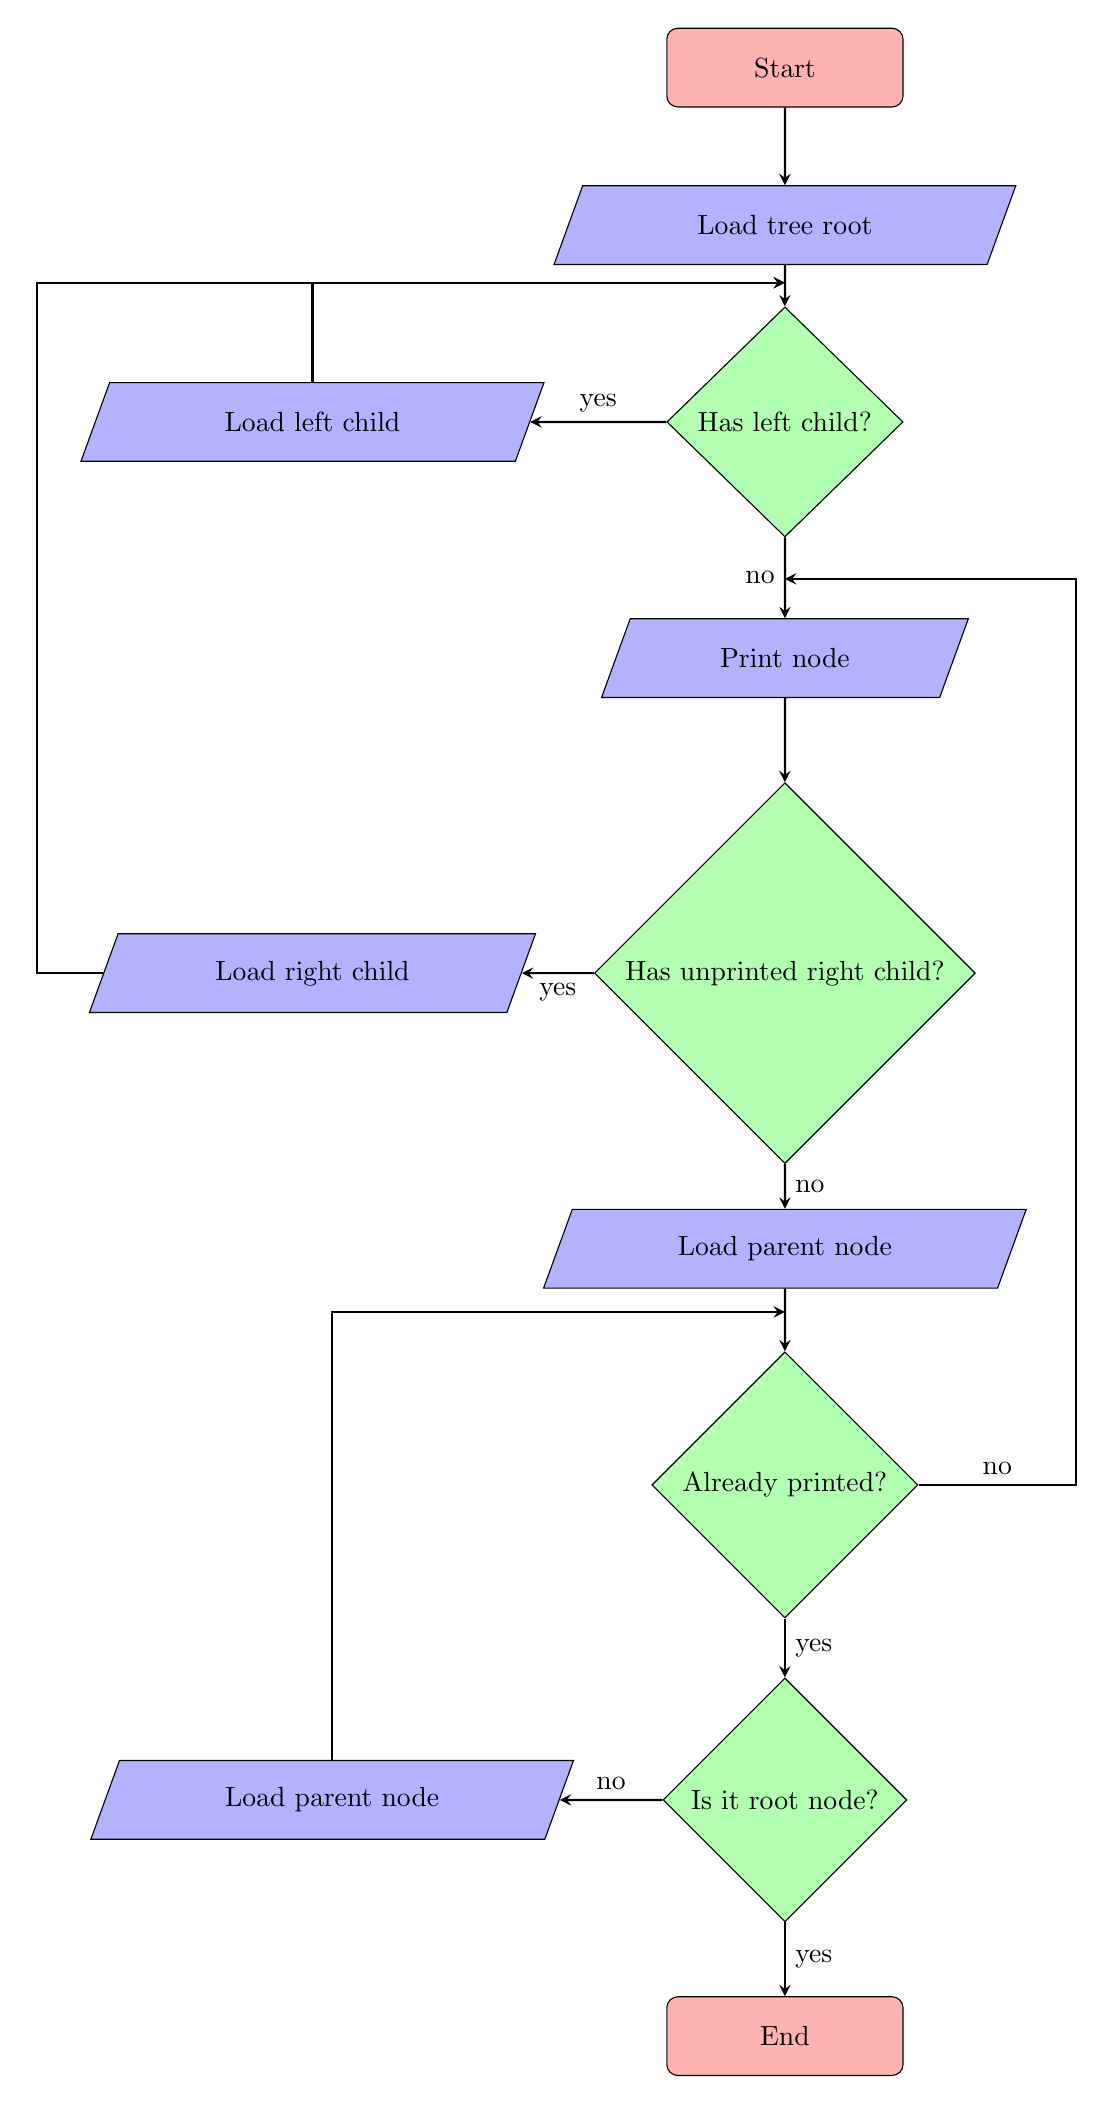
\begin{tikzpicture}[node distance=2cm]
    \node (start) [startstop] {Start};
    \node (in_root) [io, below of=start] {Load tree root};
    \node (dec1) [decision, below of=in_root, yshift=-0.5cm] {Has left child?};
    \coordinate (above dec1) at ($(dec1.north)+(0,0.3cm)$);
    \node (in_left) [io, left of=dec1, xshift=-4cm] {Load left child};
    \coordinate (above in_left) at ($(dec1.north)+(0,0.3cm)$);
    \coordinate (left_in_left) at ($(in_left.west)+(-0.3,0cm)$);
    \node (print_node) [io, below of=dec1, yshift=-1cm]{Print node};
    \node (has_right) [decision, below of=print_node, yshift=-2cm] {Has unprinted right child?};
    \node (in_right) [io, left of=has_right, xshift=-4cm] {Load right child};
    \node (in_parent) [io, below of=has_right, yshift=-1.5cm] {Load parent node};
    \node (is_printed) [decision, below of=in_parent, yshift=-1cm] {Already printed?};
    \node (is_root) [decision, below of=is_printed, yshift=-2cm] {Is it root node?};
    \node (in_parent2) [io, left of=is_root, xshift=-3.75cm] {Load parent node};
    \node (end) [startstop, below of=is_root, yshift=-1cm] {End};

    \node (node1) [left of=above dec1, xshift=-7.5cm] {};
    \gettikzxy{(node1)}{\ax}{\ay};
    \gettikzxy{(in_right.west)}{\bx}{\by};
    \coordinate (node2) at (\ax, \by);

    \coordinate (node3) at ($(is_printed.east) + (2, 0cm)$) {};
    \gettikzxy{(node3)}{\ax}{\ay};
    \gettikzxy{(print_node)}{\bx}{\by};
    \coordinate (node4) at (\ax, \by);
    \coordinate (node5) at ($(print_node.north)+(0,0.5cm)$);

    \coordinate (node6) at ($(is_printed.north)+(0,0.5cm)$);

    \draw [arrow] (start) -- (in_root);
    \draw [arrow] (in_root) -- (dec1);
    \draw [arrow] (dec1) -- node[anchor=south] {yes} (in_left);
    \draw [arrow] (dec1) -- node[anchor=east] {no} (print_node);
    \draw [arrow] (print_node) -- (has_right);
    \draw [arrow] (has_right) -- node[anchor=north] {yes} (in_right);
    \draw [arrow] (has_right) -- node[anchor=west]{no} (in_parent);
    \draw [arrow] (in_parent) -- (is_printed);
    \draw [arrow] (is_printed) -- node [anchor=west] {yes} (is_root);
    \draw [arrow] (is_root) -- node [anchor=south] {no} (in_parent2);
    \draw [arrow] (is_root) -- node[anchor=west] {yes}(end);

    \draw [arrow] (in_left.north) |- (above dec1);
    \draw [arrow] (in_right.west) -- (node2) -- (node1.south) |- (above dec1);
    \draw [arrow] (is_printed.east) -- node[anchor=south]{no}(node3) -- (node4) |- (node5);
    \draw [arrow] (in_parent2.north) |- (node6);

\end{tikzpicture}


\end{document}


